\chapter{Operations and algorithms}

\label{chap:op_al}

Our aim in this chapter is to describe algorithms over 3D data structures. In each description of
an algorithm there is a short paragraph that summarizes required operations for running the algorithm.
It is later used in hierarchical implementation of the algorithms.\\
\\
The article\cite{Grunbaum2007} proves that the mesh representation of a hole-free solid object can be
treated as planar graph, and a polygon mesh as general unoriented graph. Therefore, we can generalize the
editing functions over polygon meshes as the operations over the graphs.\\

\section{Euler operators}
\label{sec:euler}

The \emph{Euler operators} are the set of operators which create a polygon meshes. One of the advantages
of these operators is that they are invertible. In the following description paragraphs,
each operator is followed by its inverted operator.

\subsection{Make Vertex}

The operation creates a vertex with no topological dependencies. It can be used
either on empty mesh or mesh with already created topology.

\begin{figure}[h]
\centering
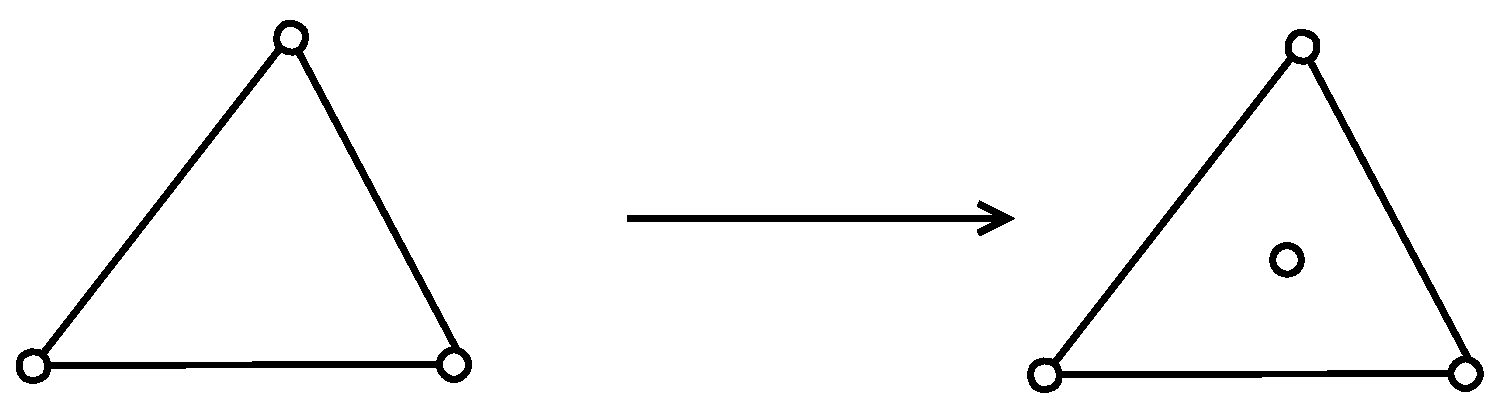
\includegraphics[scale=0.25]{../img/makeV.eps}
\label{fig:makev}
\caption{Euler operator makeV}
\end{figure}

\subsection{Kill Vertex}

The operation removes a vertex that is required not to be contained in faces or
edges.

\begin{figure}[h]
\centering
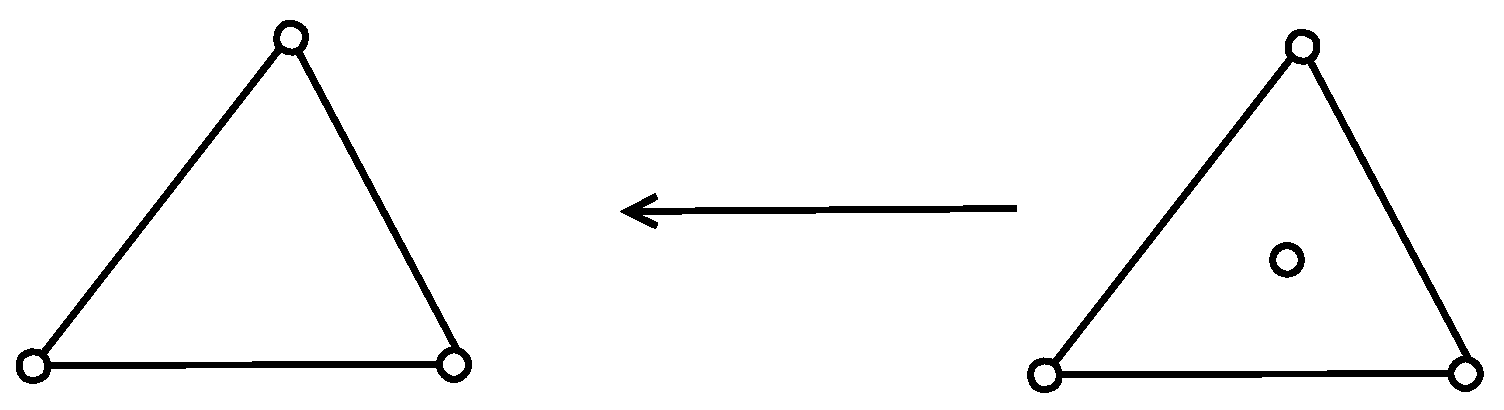
\includegraphics[scale=0.25]{../img/killV.eps}
\label{fig:killv}
\caption{Euler operator killV}
\end{figure}


\subsection{Make Vertex and Edge}

The operation \emph{Make Vertex and Edge} creates a vertex and connects
it with an another vertex that is already contained in the mesh.

\begin{figure}[h]
\centering
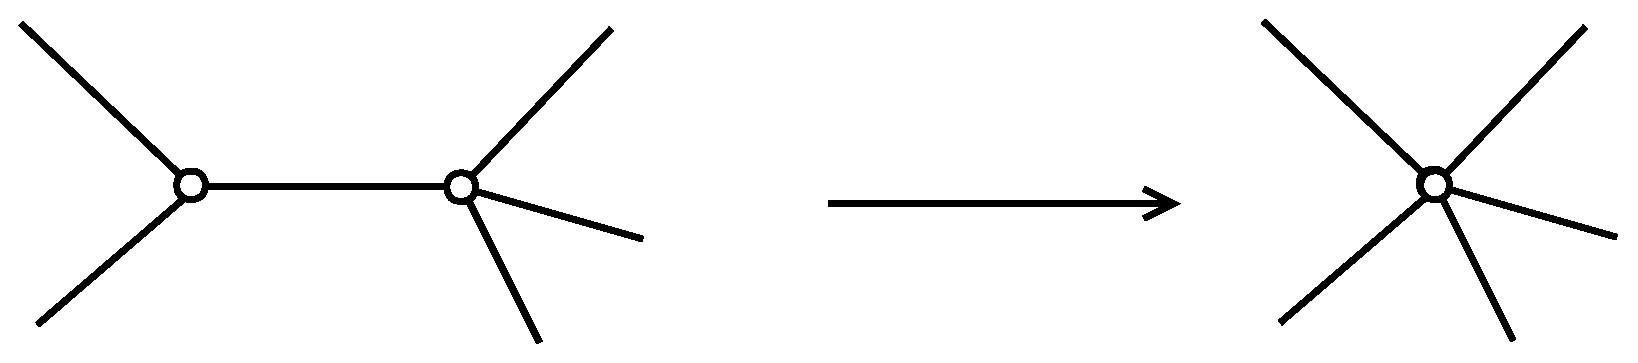
\includegraphics[scale=0.25]{../img/makeEV.eps}
\label{fig:makeev}
\caption{Euler operator makeEV}
\end{figure}

\subsection{Kill Vertex and Edge}

It removes a vertex and disposes the edge that is connected to the vertex.

\begin{figure}[H]
\centering
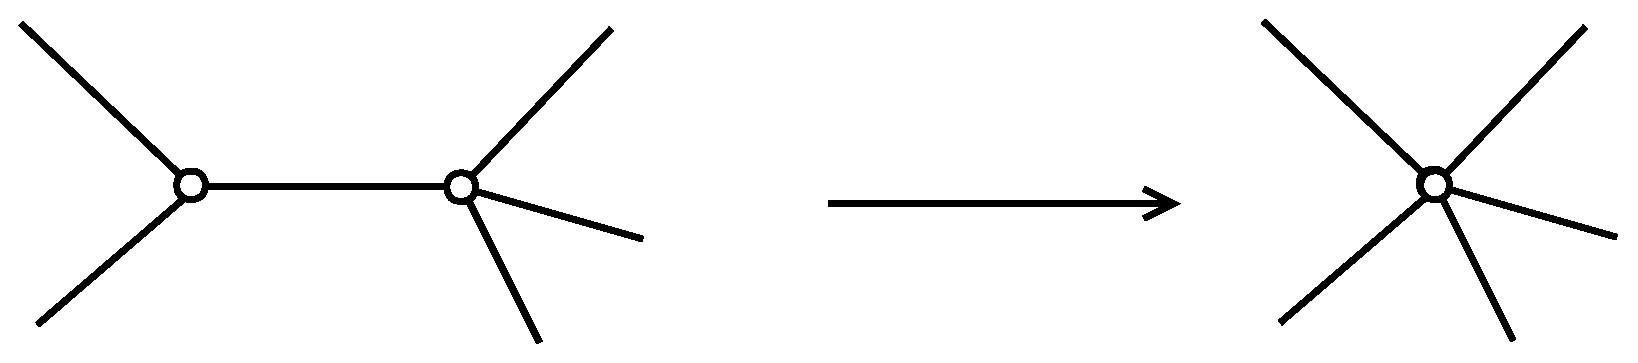
\includegraphics[scale=0.25]{../img/killEV.eps}
\label{fig:killev}
\caption{Euler operator killEV}
\end{figure}

\subsection{Make Edge and Face}

This operation creates an edge and forms a new face by splitting another one, or by forming a new
face.

\begin{figure}[H]
\centering
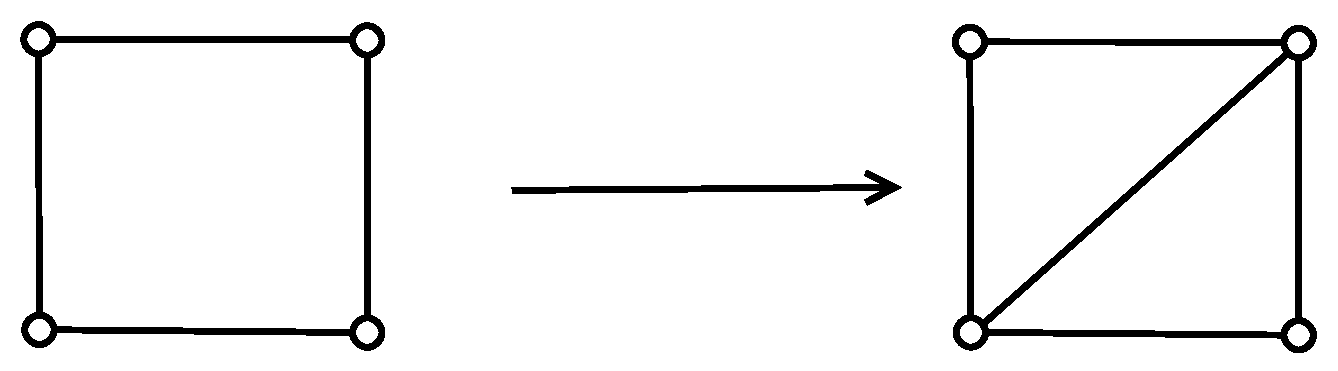
\includegraphics[scale=0.25]{../img/makeEF.eps}
\label{fig:makeef}
\caption{Euler operator makeEF}
\end{figure}

\subsection{Kill Edge and Face}

It removes the edge and the face that is connected to the edge.

\begin{figure}[H]
\centering
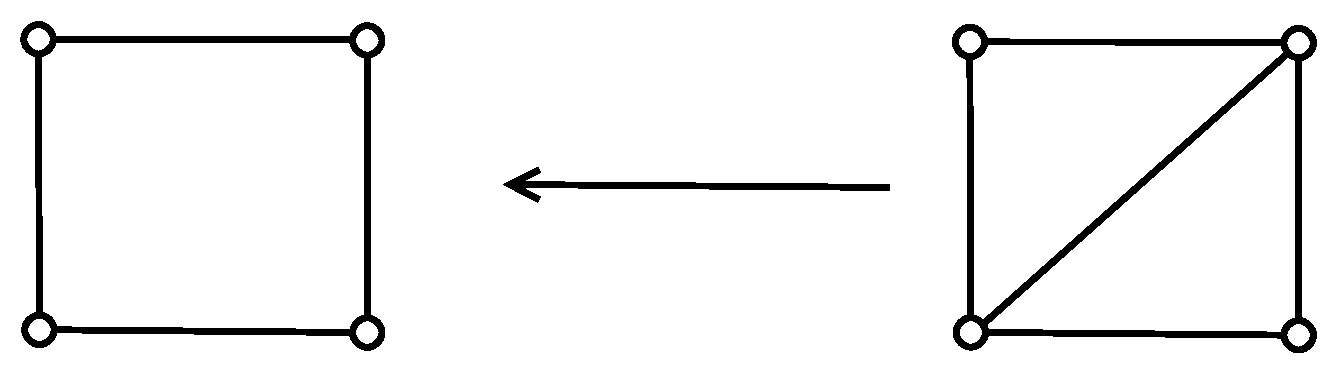
\includegraphics[scale=0.25]{../img/killEF.eps}
\label{fig:killef}
\caption{Euler operator killEF}
\end{figure}

\subsection{Make Face and Kill Ring}

It creates a face by disposing the ring because of the addition of a new edge.

\begin{figure}[H]
\centering
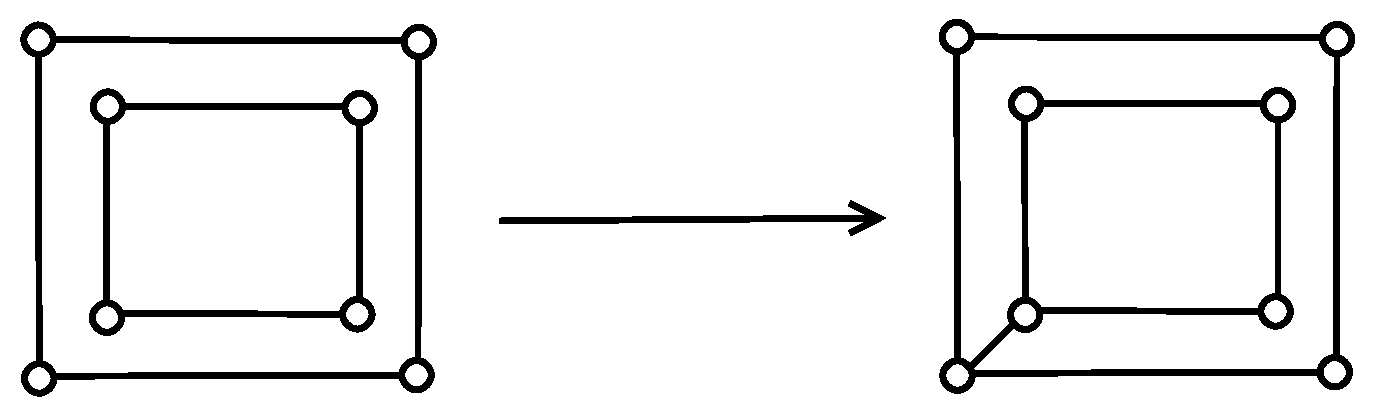
\includegraphics[scale=0.25]{../img/makeFkillR.eps}
\label{fig:makefkillr}
\caption{Euler operator makeFkillR}
\end{figure}

\subsection{Kill Face and Make Ring}

The operation creates a ring by disposing a face.

\begin{figure}[H]
\centering
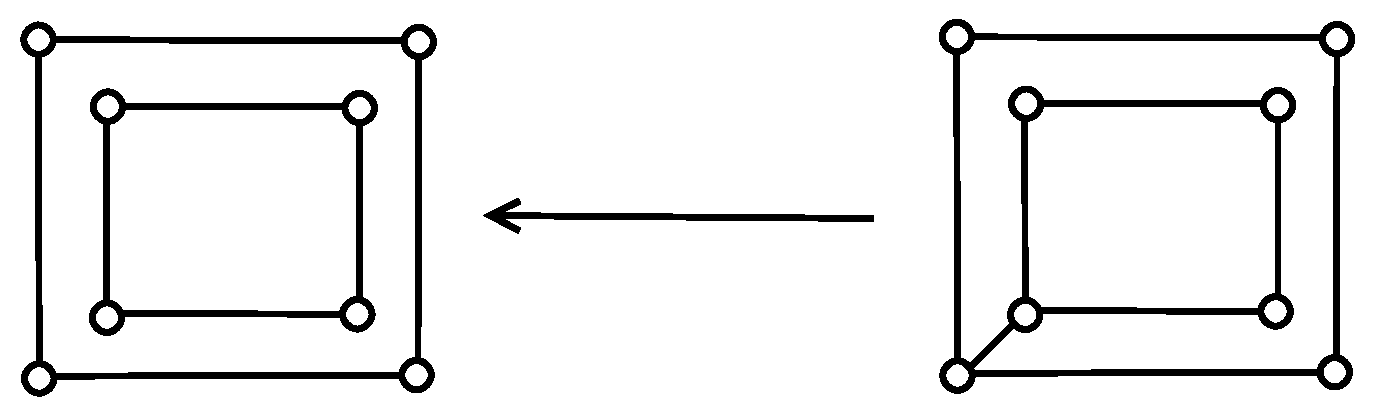
\includegraphics[scale=0.25]{../img/killFmakeR.eps}
\label{fig:killfmaker}
\caption{Euler operator killFmakeR}
\end{figure}


\section{Editing functions}
\label{sec:edit_f}
Some functions are designed to change size or shape of the object. Those functions are called 
\emph{editing function}.
During the editing of the object, the user defines required values and the function deforms the
object properly. In case of the editing function \emph{scaling} for instance, a user defines the scaling
ratio.

\subsection{Truncate}

Truncate is the operation that affects a topology of a mesh. From a given vertex, it creates a new face with
surroundings of the original vertex. This is a common operation of mesh editing used e.g. in
3D editors.\\

\begin{figure}[ht]
\centering
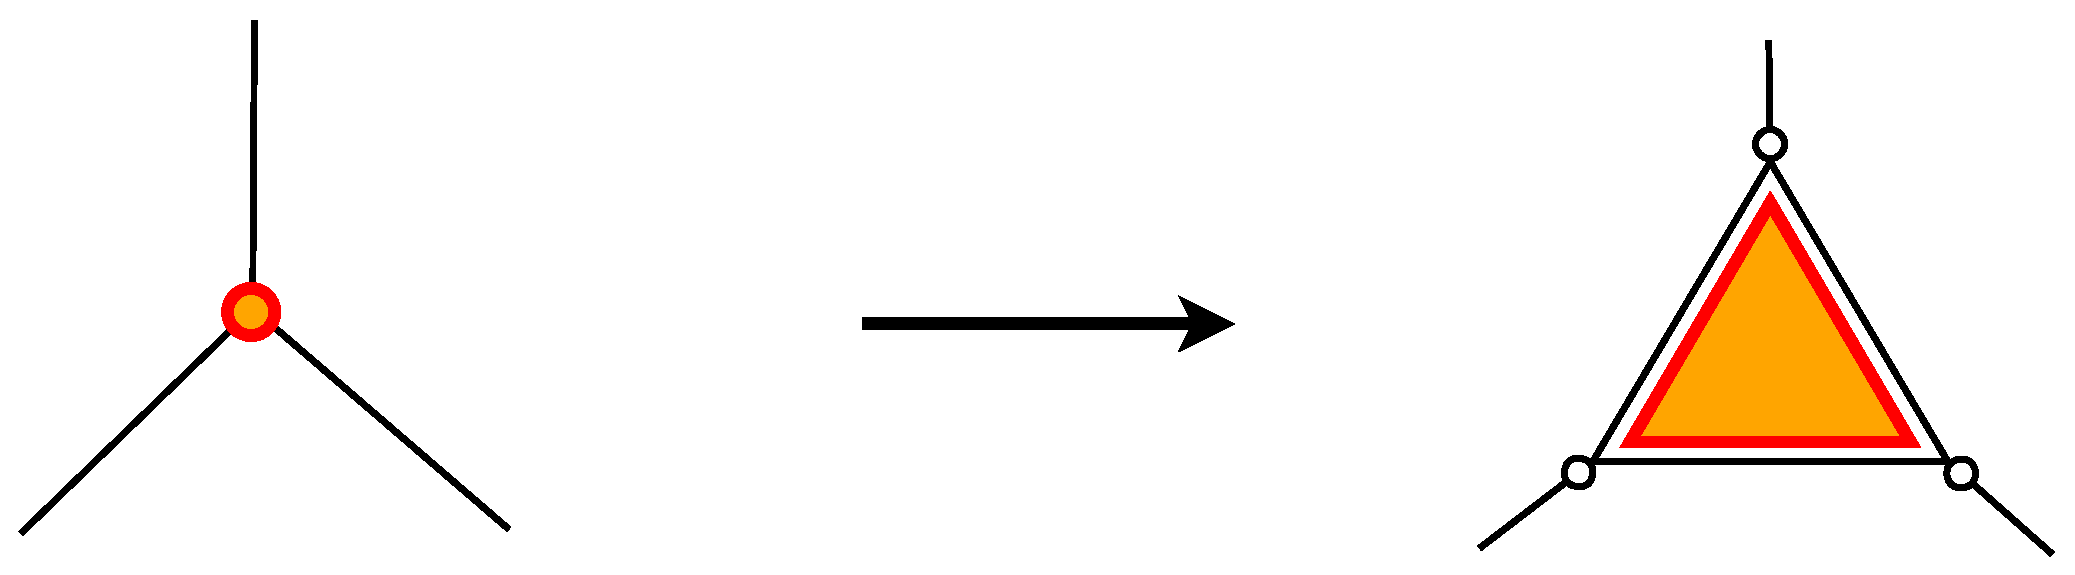
\includegraphics[scale=0.2]{../img/truncate.eps}
\caption{The red-marked vertex is a selected vertex to be truncated.
The face filled by the orange color with the red borders is the resulting face created by the truncation}
\end{figure}

\subsection{Bevel}

This operation is almost identical with the \emph{truncation}. The only difference is the argument of the
operation. As the truncate operation creates a new face based on the given vertex, the bevel operation
creates the face from a given edge.\\

\begin{figure}[ht]
\centering
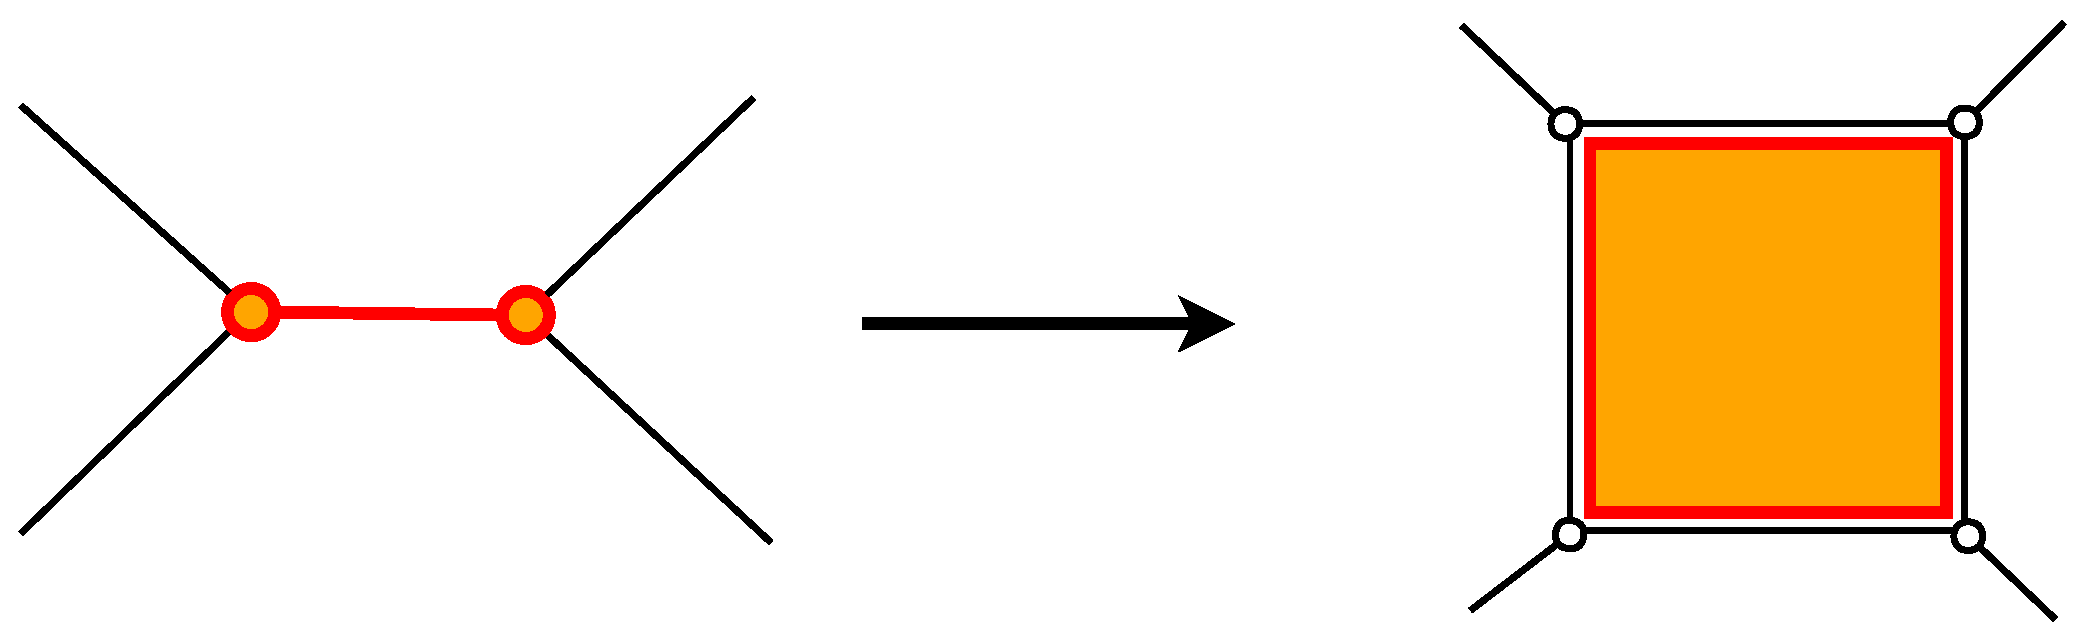
\includegraphics[scale=0.2]{../img/bevel.eps}
\caption{The red-marked edge is a selected edge to be beveled. As in the previous case, the resulting
face is filled by the orange color.}
\end{figure}

\subsection{Extrude}

In the previous operations the argument is a vertex and then an edge. Intuitively, one can assume
that there is an operation that demands a face as the argument. Operation \emph{extrude} ``pulls"
the face out the object creating new faces connecting the extruded face with the resulting object.

\begin{figure}[ht]
\centering
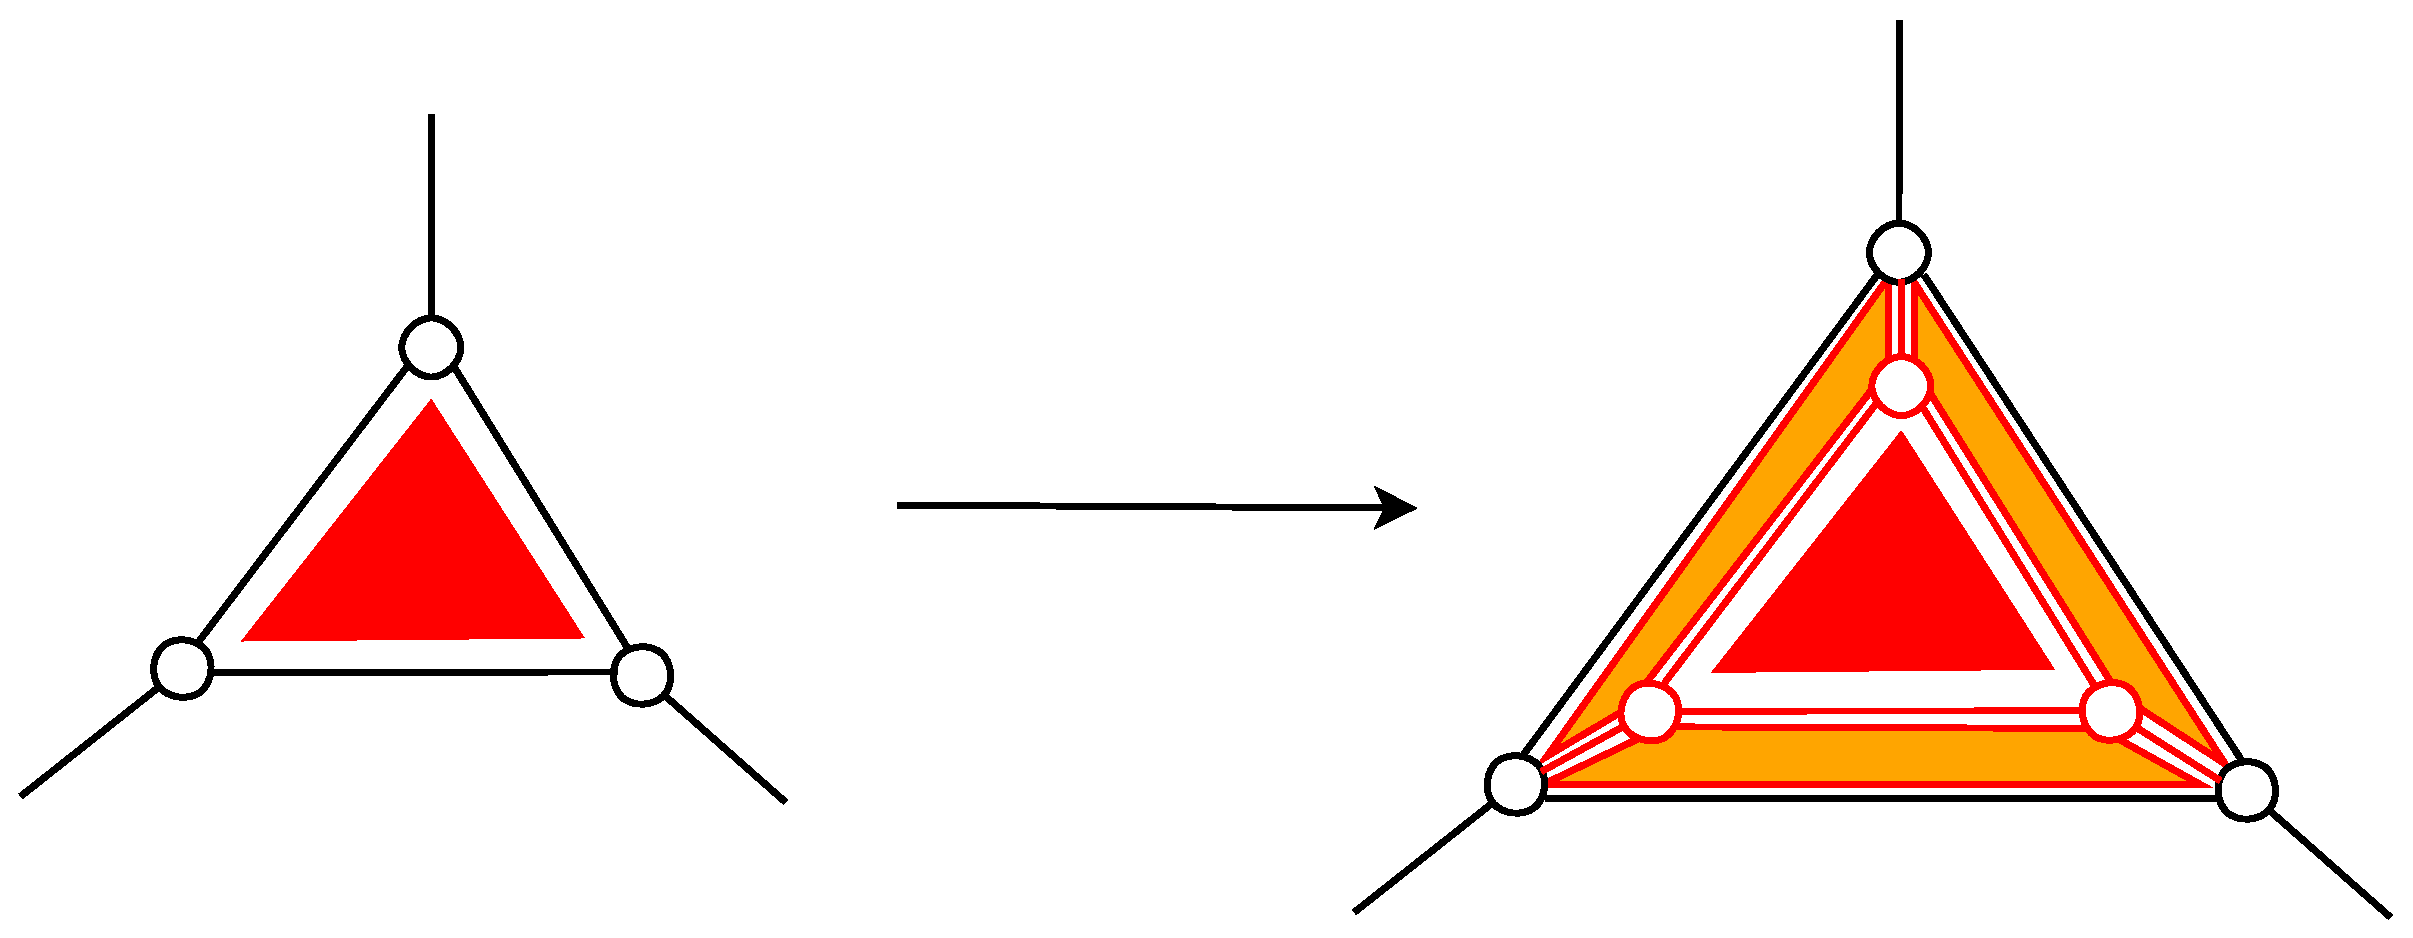
\includegraphics[scale=0.2]{../img/extrude.eps}
\caption{The red-filled face is a selected face to be extruded. The operation creates a set of
faces (marked with orange) with the topology as shown on the picture.}
\end{figure}

\section{Converting between representations}

In this section introduces some algorithms that convert one representation to another. Each 
representation has its own capability.

\subsection{Delaunay triangulation}

Let $P$ be a set of points in the $d$-dimensional Euclidean space.
Delanuay triangulation is triangulation such that no point $p \in P$ is inside the circum-hypersphere
of any simplex in $DT(P)$. For better imagination, in case of $2$-dimensional space, no point
structure is inside the circumcircle of any triangle of resulting structure.

\subsection{Marching cubes}
\label{sub:march}

Marching cubes algorithm converts a grid representation to a mesh \cite{Lorensen1987}. It iterates through
all grid elements and builds a new polygonial mesh. For each element (that can be considered as
\emph{cube}, cuboid or even parallelepiped)
it determines whether the corners are inside or outside object. The algorithm considers only those elements
which contain both categories of points; rest of them are ignored. As each element has 8 corners,
each of them can be determined either as inside or outside object. In result, the element can possibly
have one of $2^8 = 256$ configurations. However, some configurations can fit to another one after rotation,
reflective simmetry, or sign changed case.\\


\begin{figure}[ht]
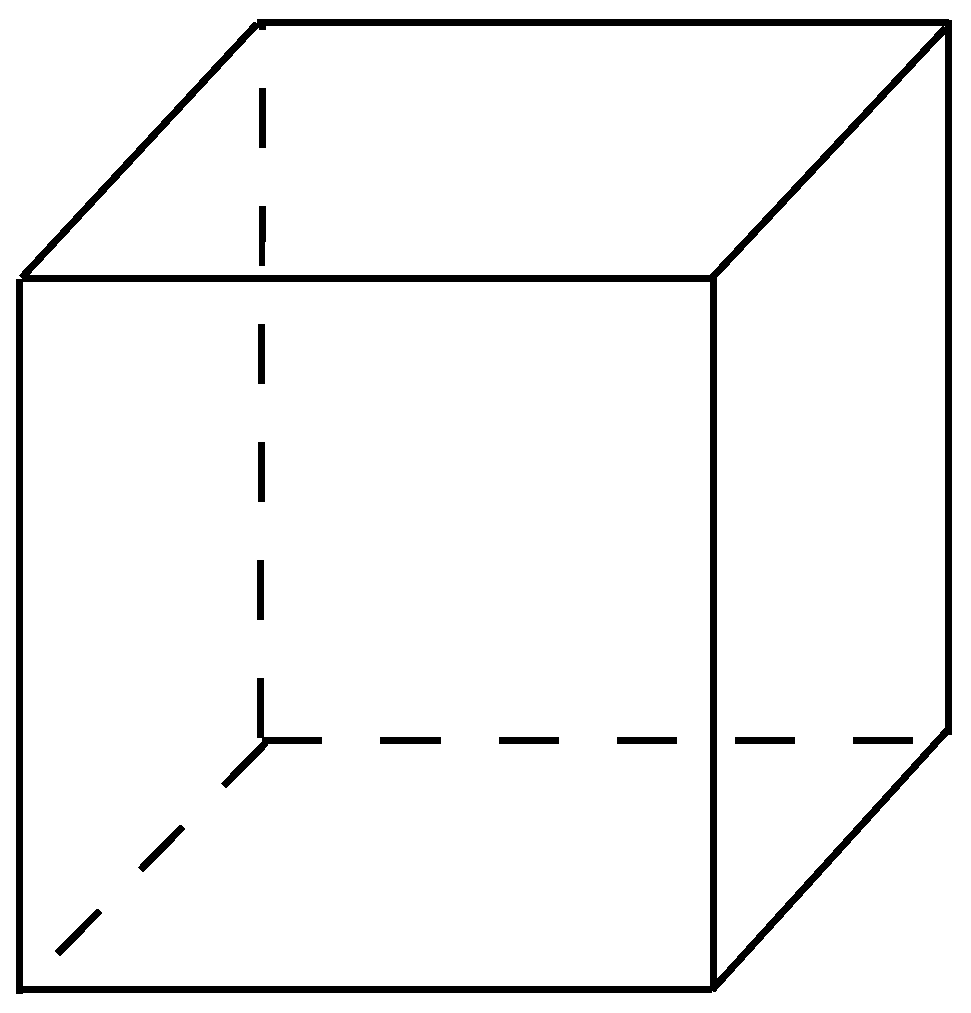
\includegraphics[scale=0.15]{../img/mar_cub_case0.eps}
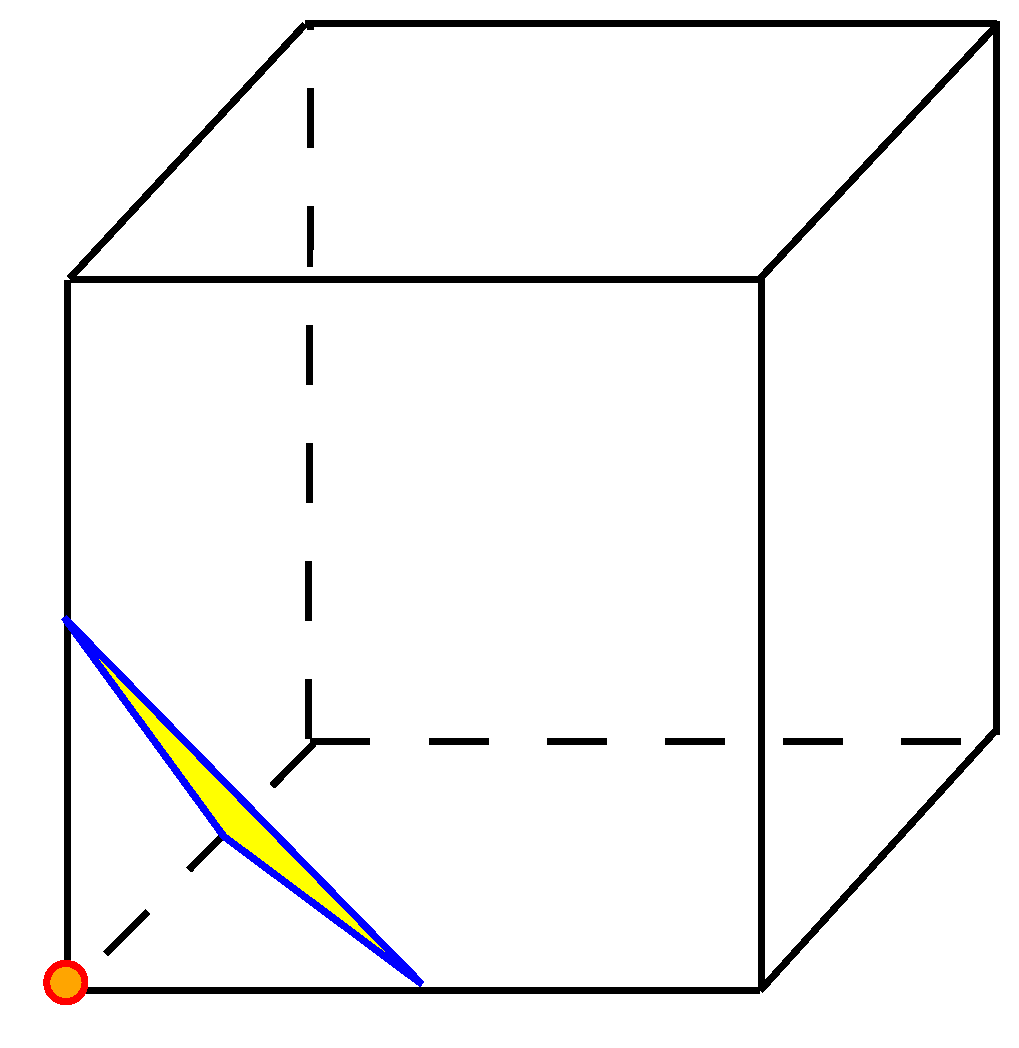
\includegraphics[scale=0.15]{../img/mar_cub_case1.eps}
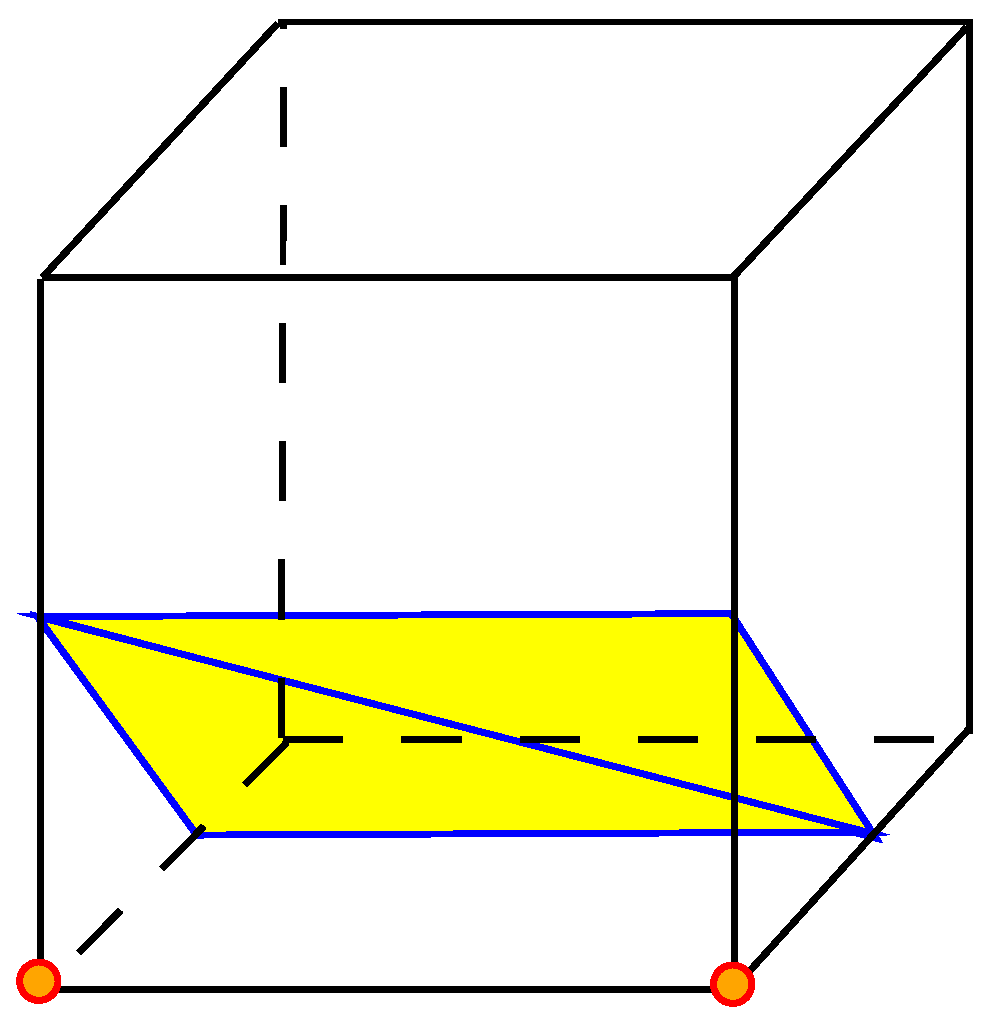
\includegraphics[scale=0.15]{../img/mar_cub_case2.eps}
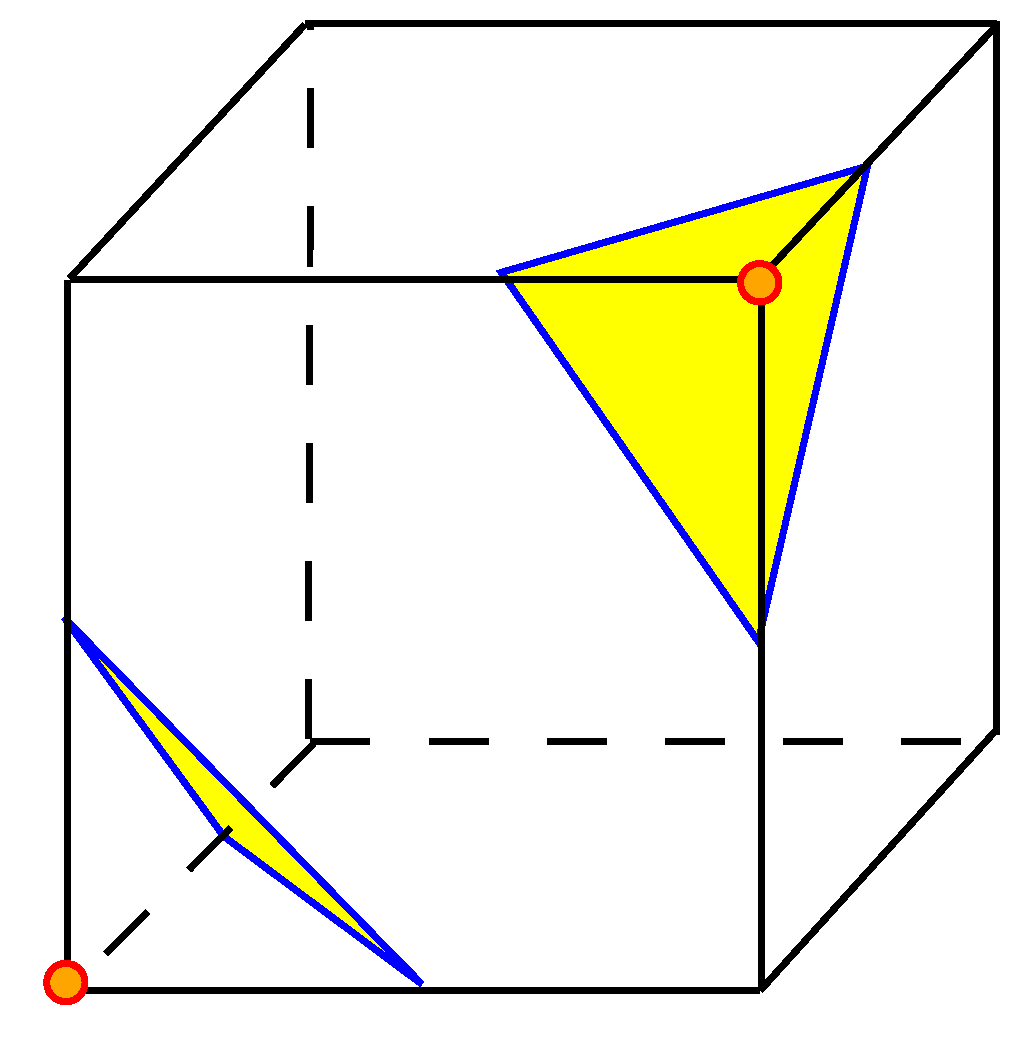
\includegraphics[scale=0.15]{../img/mar_cub_case3.eps}
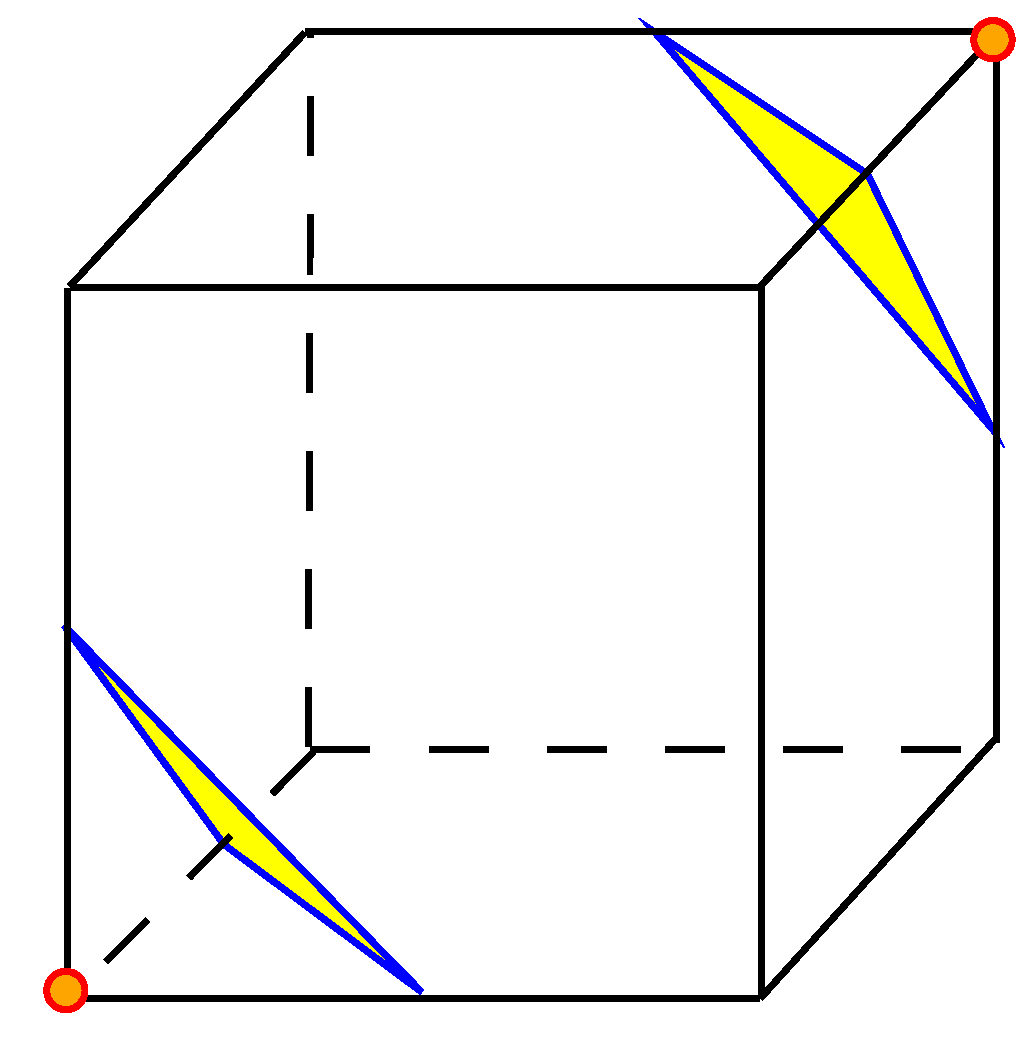
\includegraphics[scale=0.15]{../img/mar_cub_case4.eps}
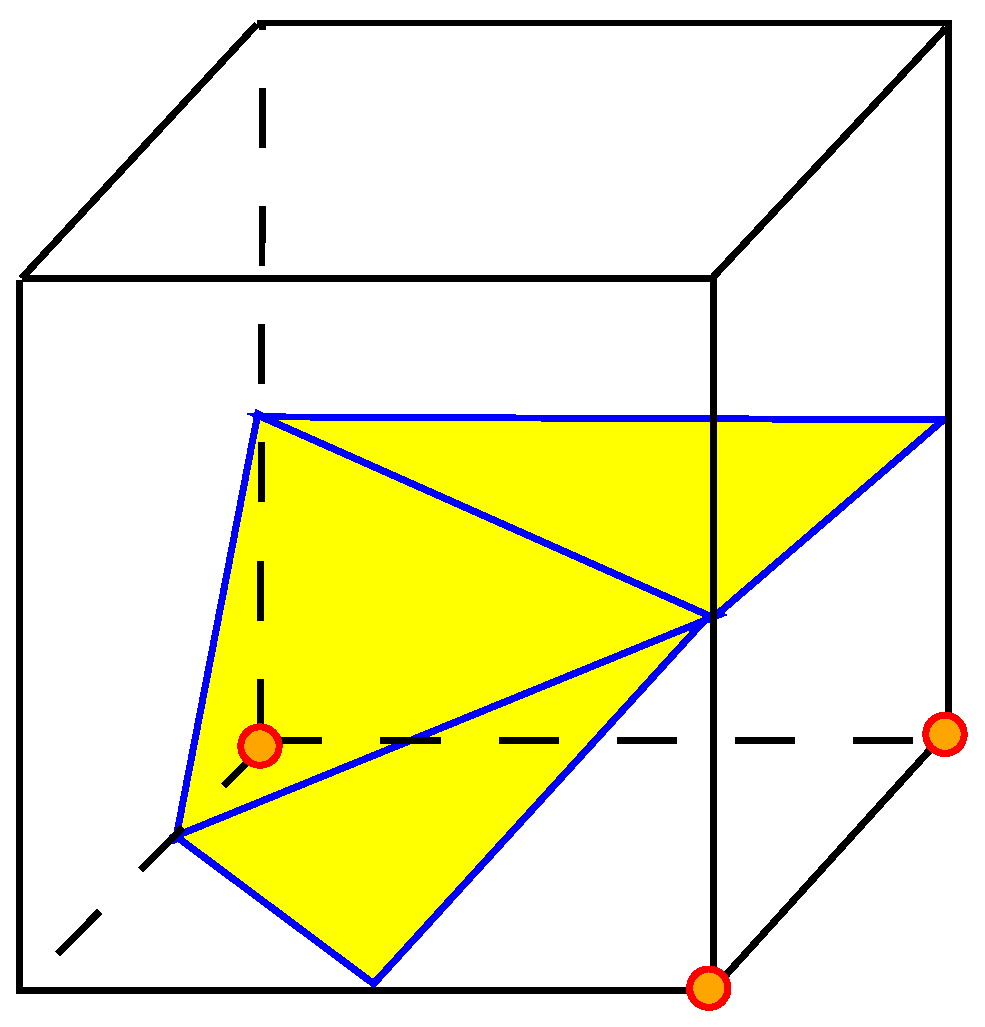
\includegraphics[scale=0.15]{../img/mar_cub_case5.eps}
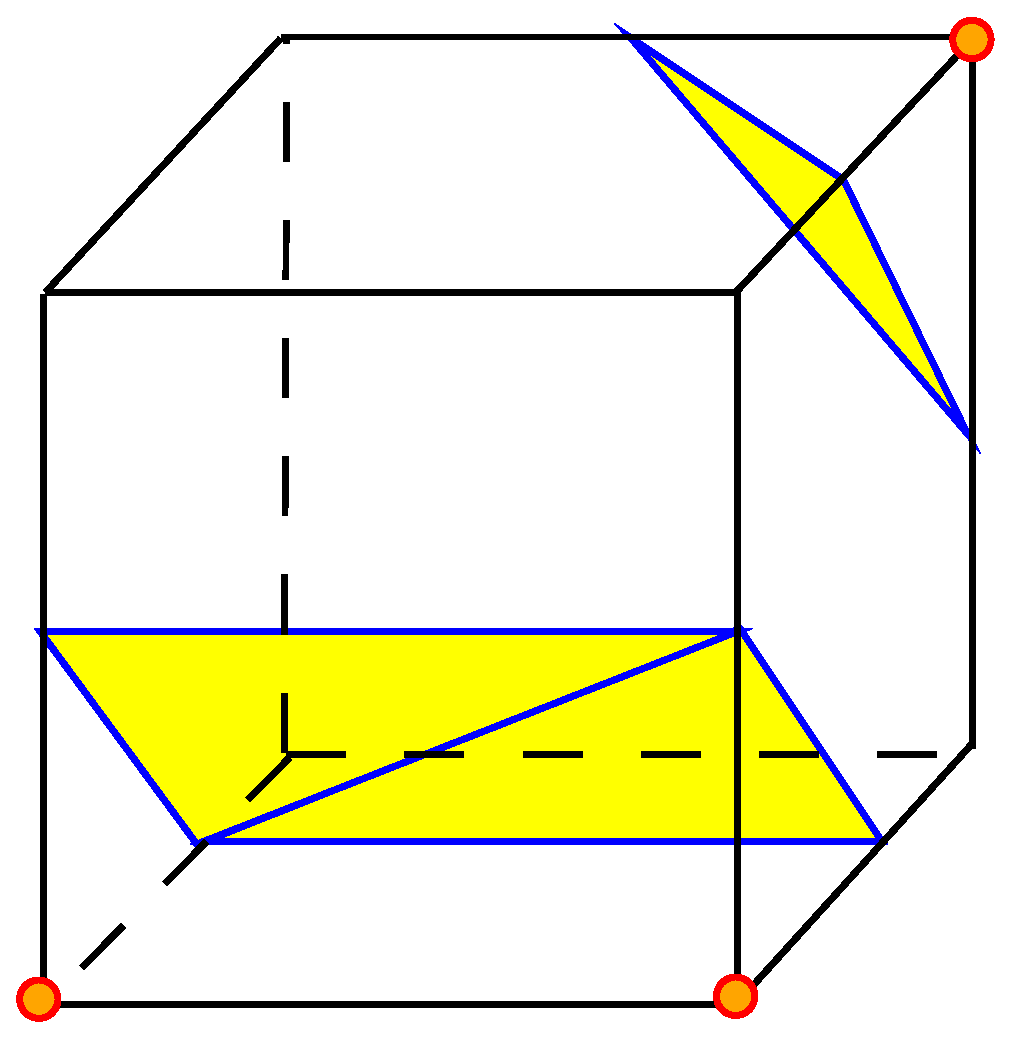
\includegraphics[scale=0.15]{../img/mar_cub_case6.eps}
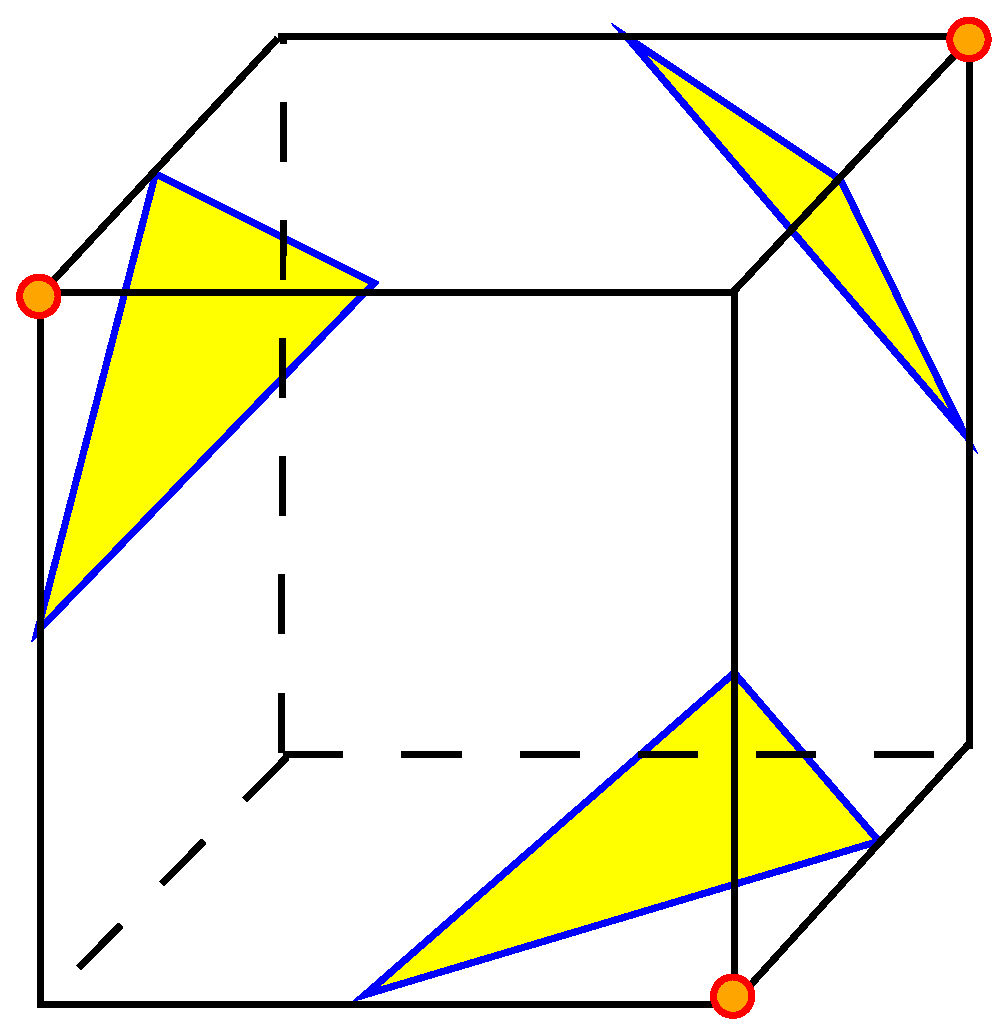
\includegraphics[scale=0.15]{../img/mar_cub_case7.eps}
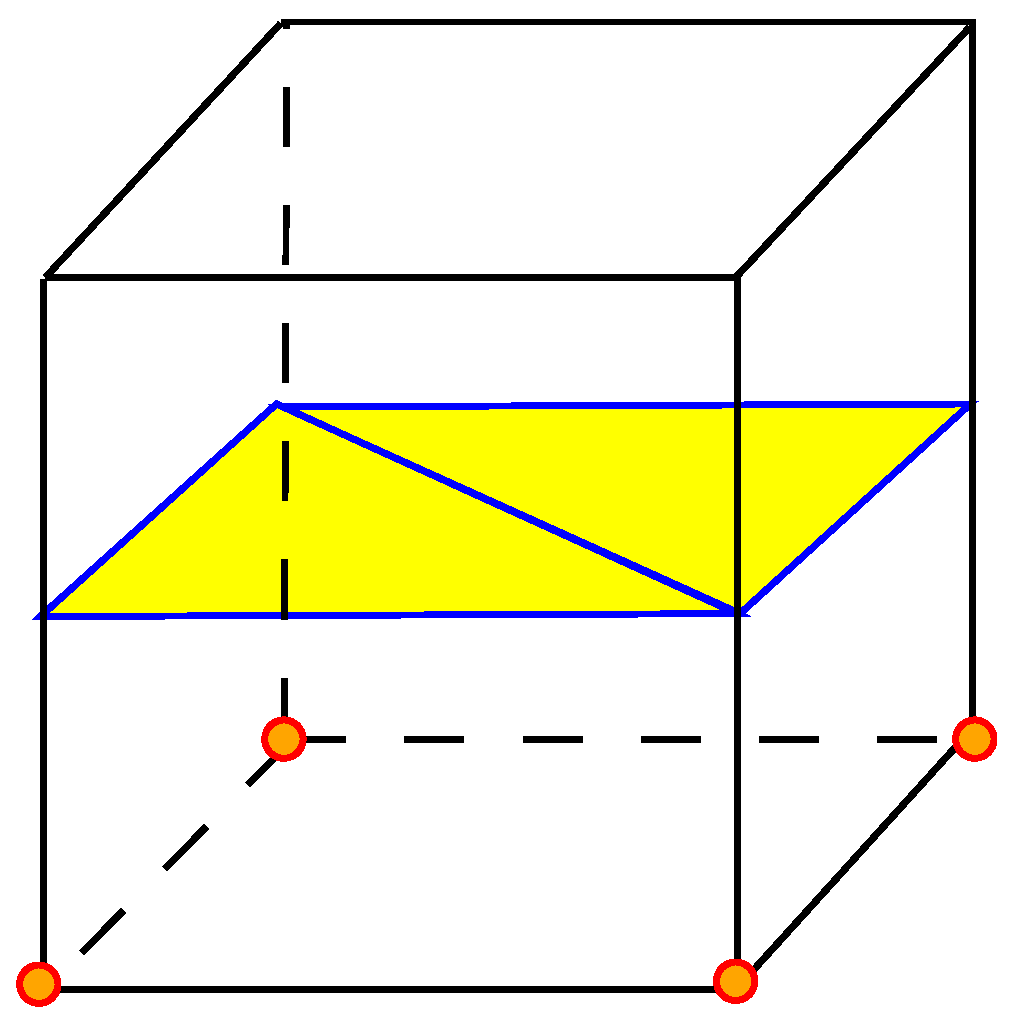
\includegraphics[scale=0.15]{../img/mar_cub_case8.eps}
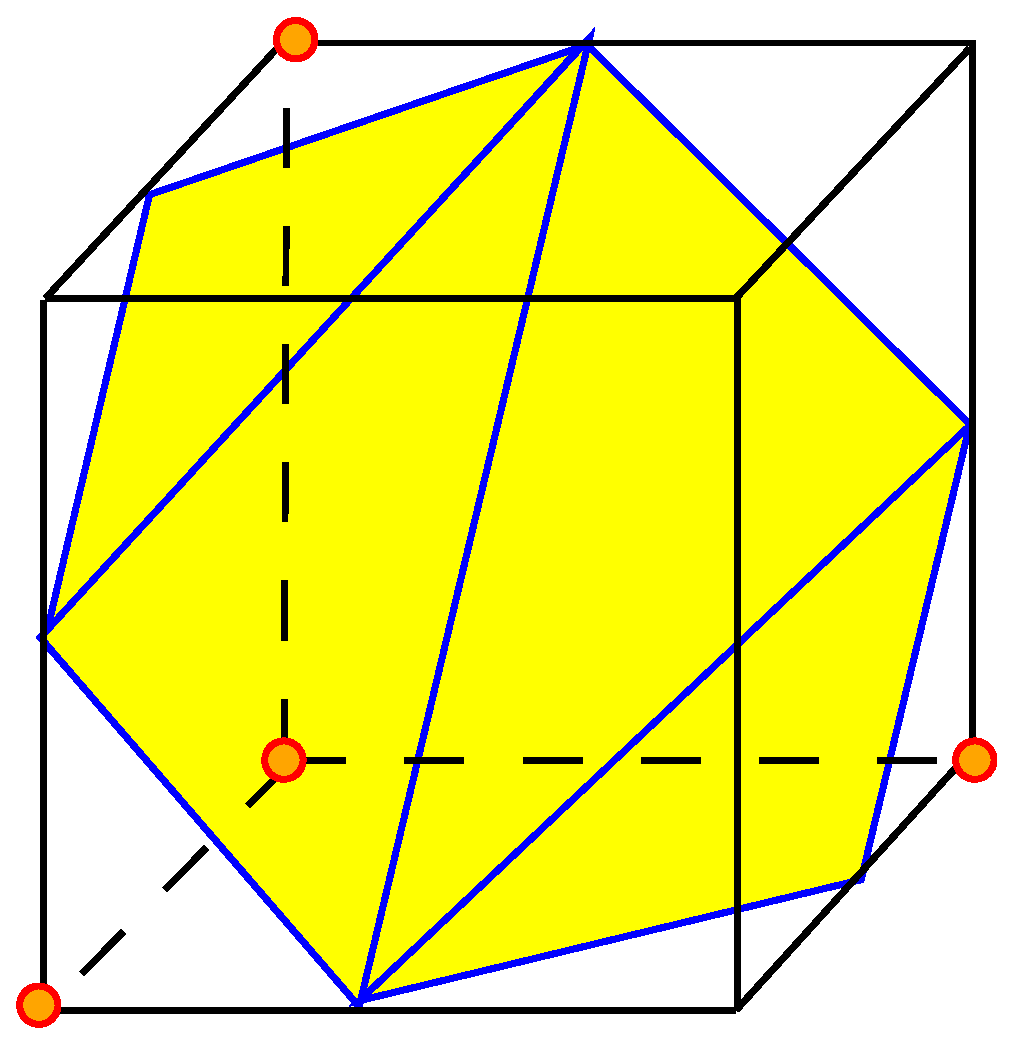
\includegraphics[scale=0.15]{../img/mar_cub_case9.eps}
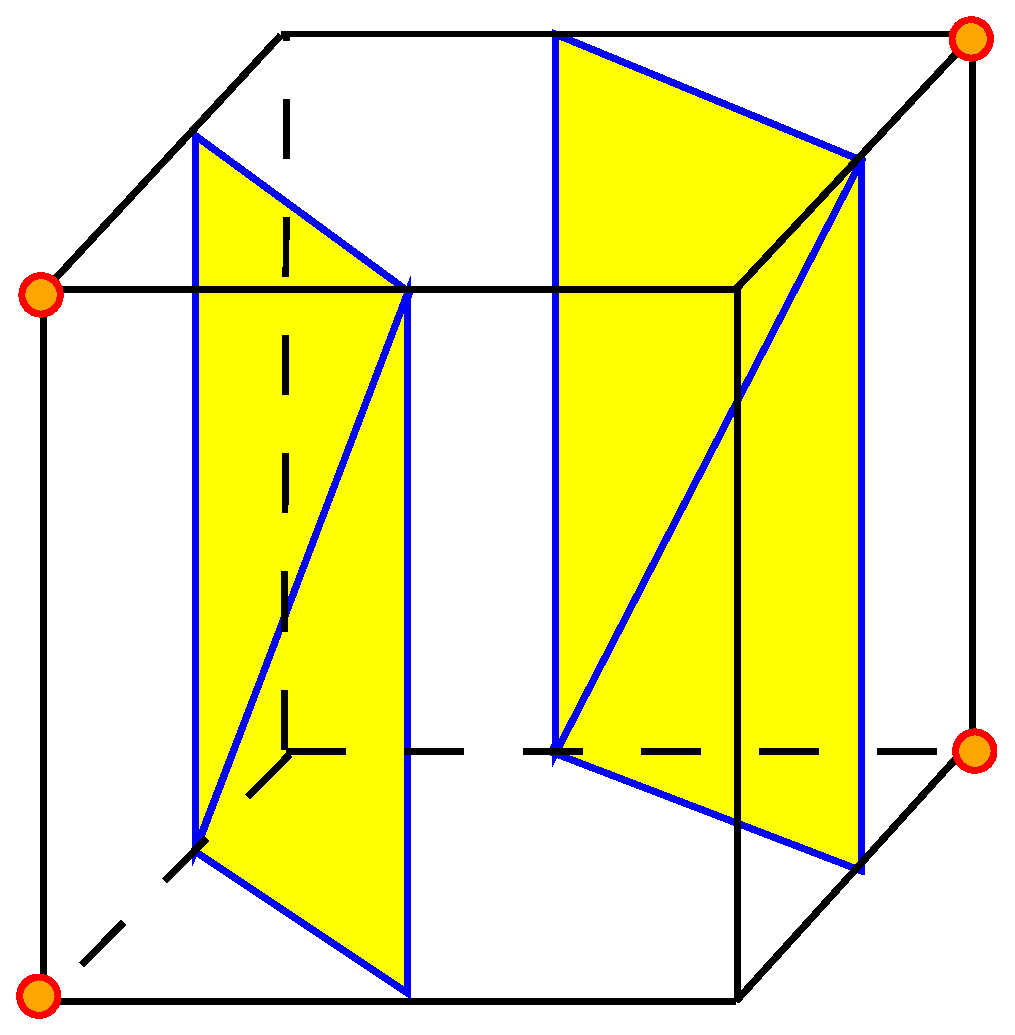
\includegraphics[scale=0.15]{../img/mar_cub_case10.eps}
\hspace{1mm}
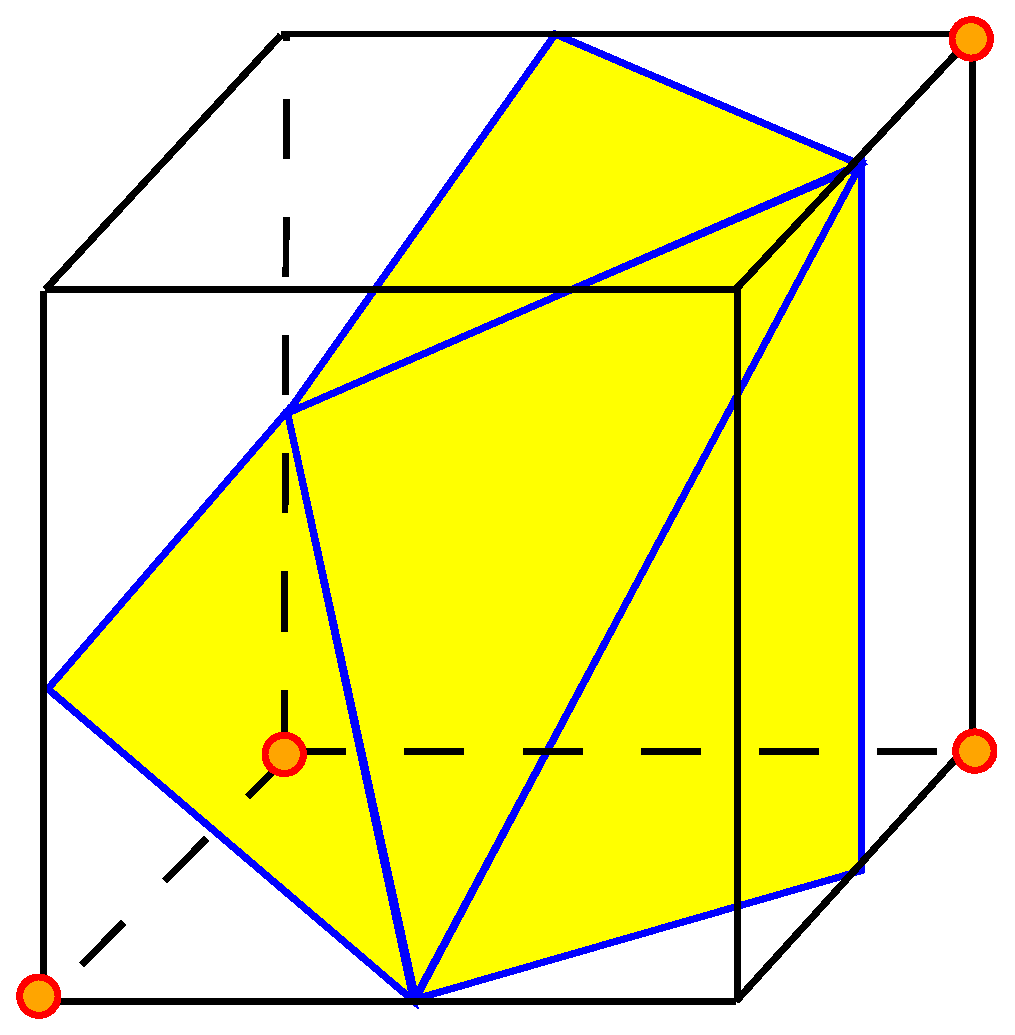
\includegraphics[scale=0.15]{../img/mar_cub_case11.eps}
\hspace{2mm}
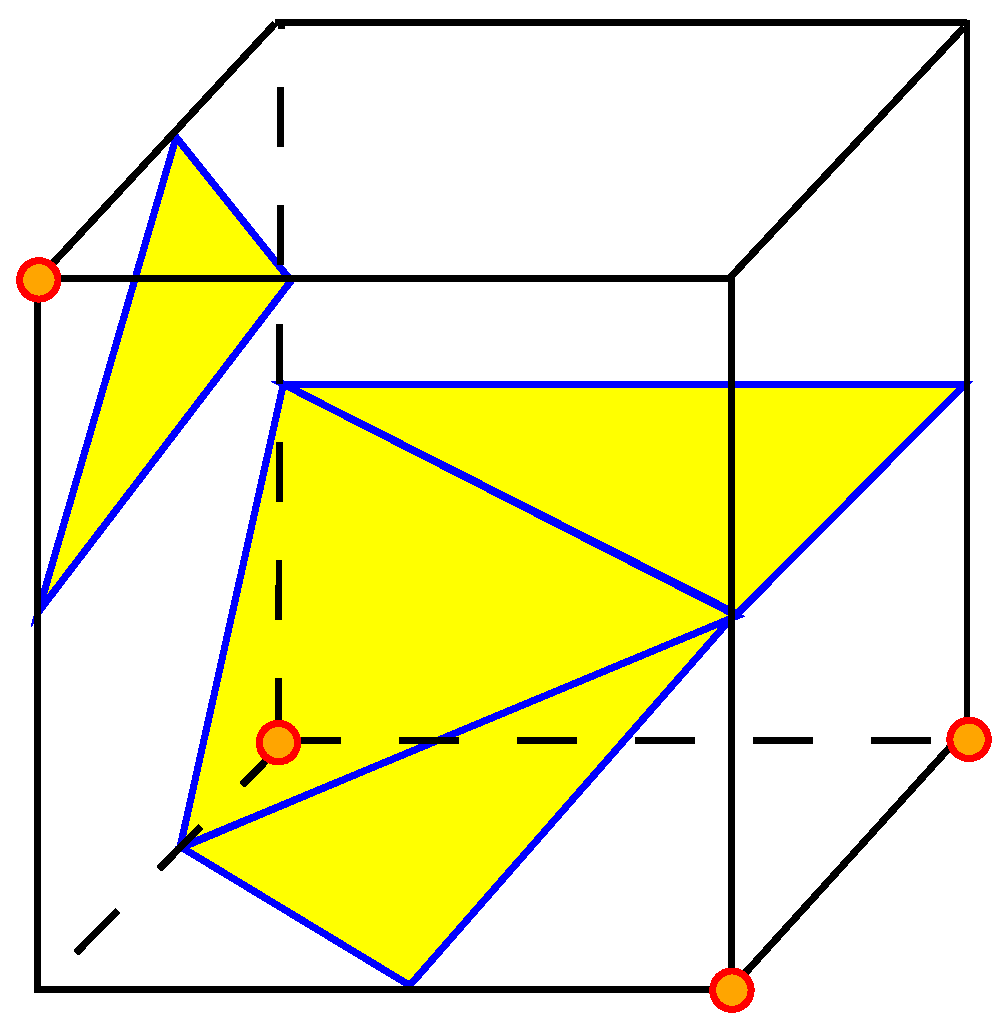
\includegraphics[scale=0.15]{../img/mar_cub_case12.eps}
\hspace{2mm}
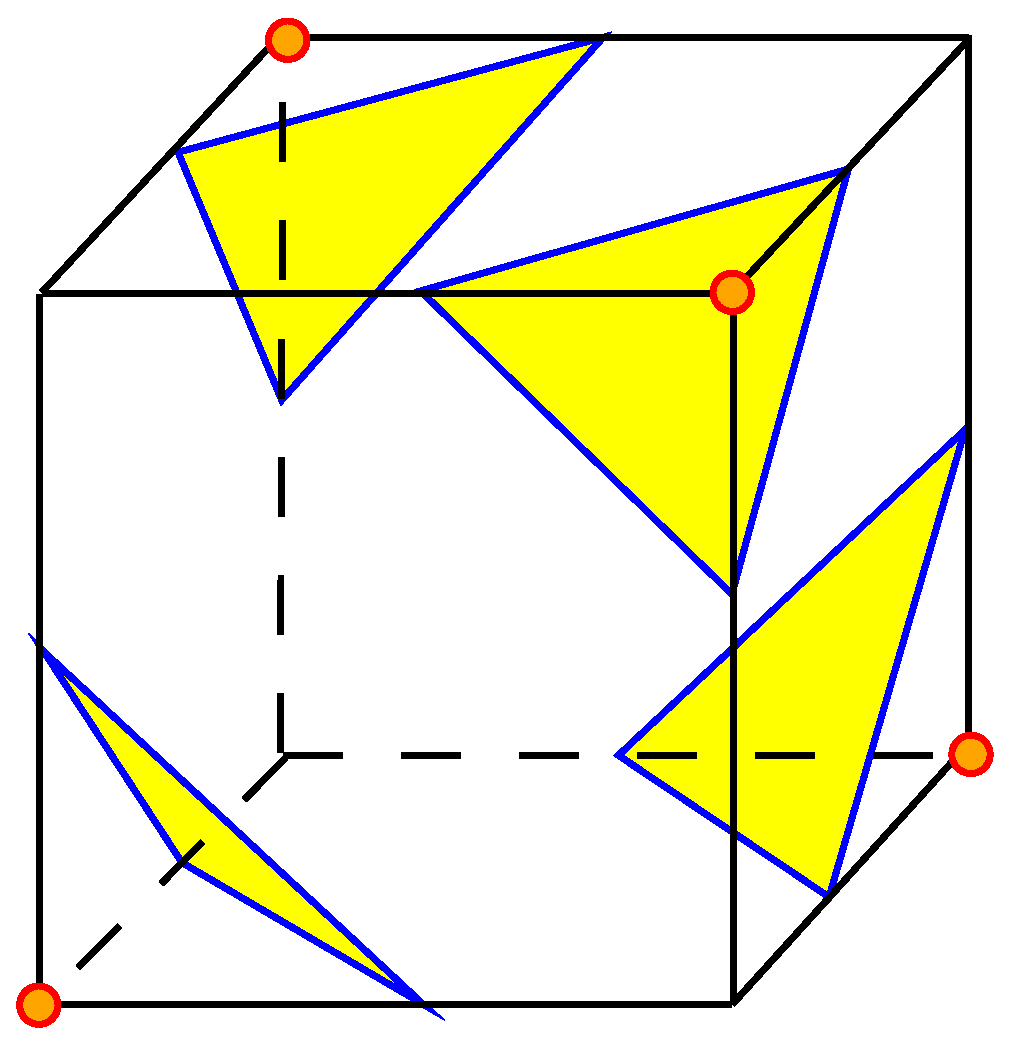
\includegraphics[scale=0.15]{../img/mar_cub_case13.eps}
\hspace{3mm}
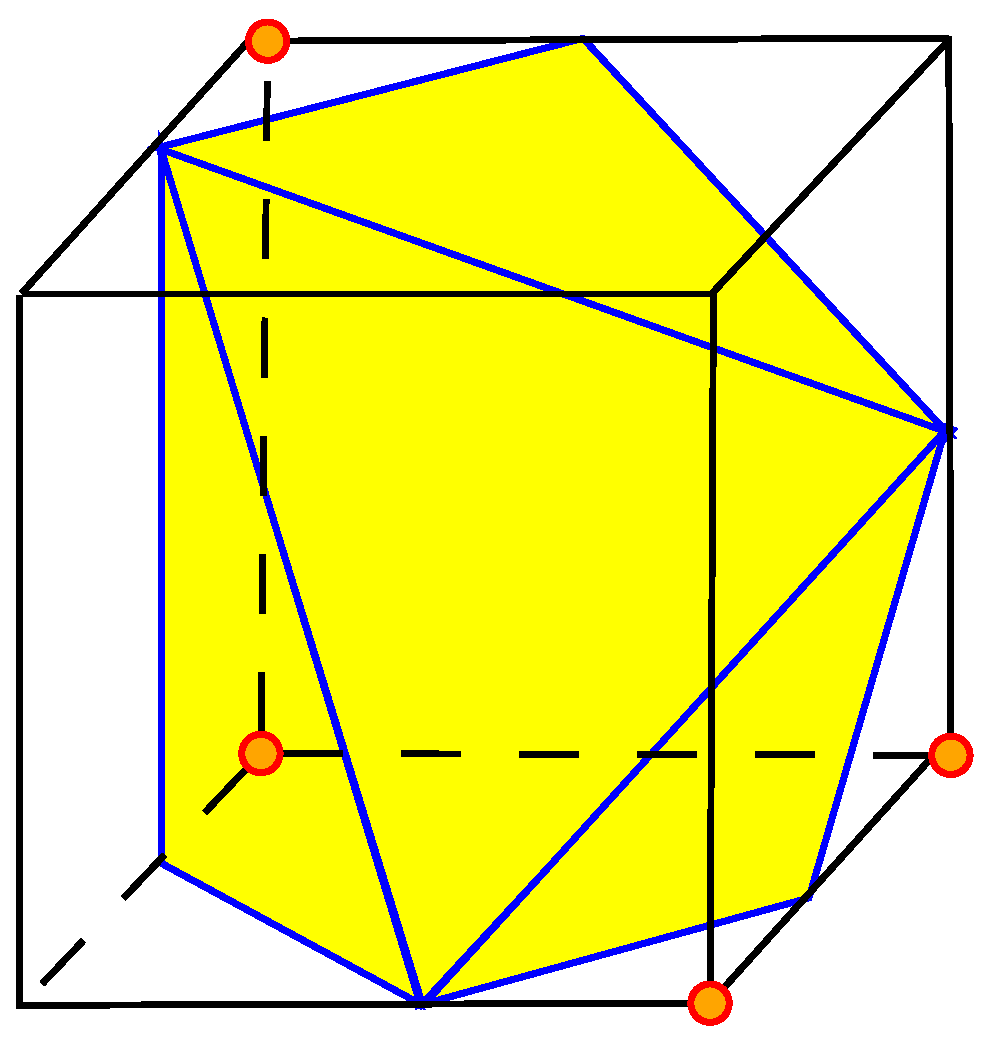
\includegraphics[scale=0.15]{../img/mar_cub_case14.eps}

\caption{The 15 cases of marching cubes algorithm. The corners that are evaluated as inside of the object
are labeled with red. The yellow triangles represent faces to be added to a mesh.}
\label{fig:mc_cases}
\end{figure}

Finaly, all of them can be reduced to $15$ unique cases. The main idea of this algorithm is to
place a set of faces for each cube in order to create a polygonal mesh with a corresponding shape.
In other words, each configuration refers to the configuration of new faces to be added to a mesh.
However, we know that two adjoining elements share 4 corners, so the resulting faces are certainly
continuous.
If the corners contain any other information, except inside/out information, the position of 
the faces in the mesh can be refined. Usually, it contains the information about a color or
the distance from point to surface. In that case, placing or any other processing of
the face is based on linear interpolation of corner values.\\
\\

\begin{figure}[!htbp]
\centering
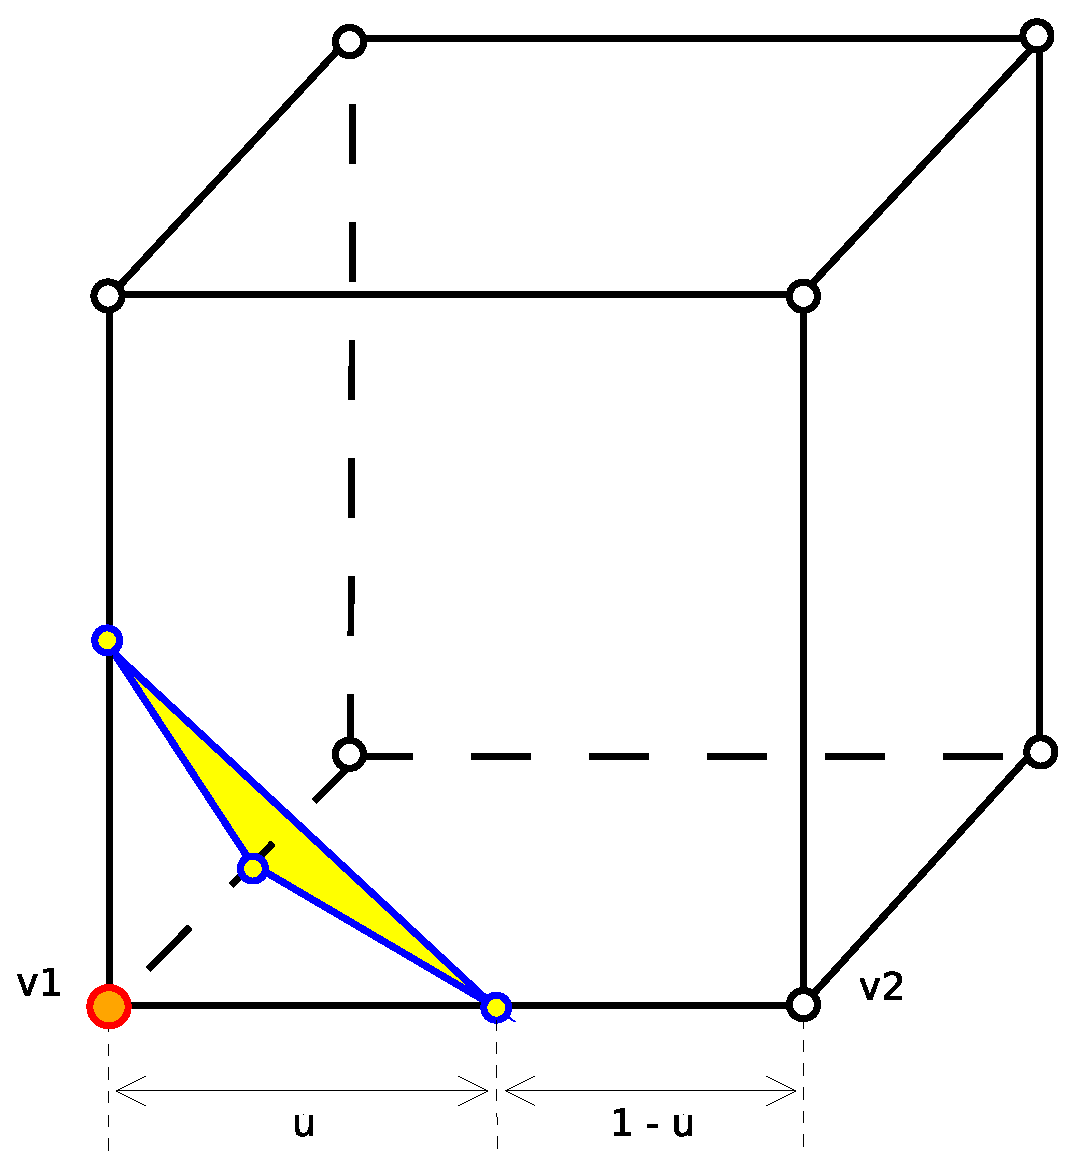
\includegraphics[scale=0.35]{../img/marc_cub_inter.eps}
\label{fig:mc_interpolation}
\caption{Interpolated position of face}
\end{figure}

Let $v1$ and $v2$ be the values that represent the distances from the surface to the corners.
Thus, we can calculate the value of coefficient $u$ from the following equation.

\begin{equation}
u = \frac{v1}{v1-v2}
\end{equation}

%This algorithm requires the capability of voxel map (or any other grid-aligned data structure) to
%determine corners configurations of arbitrary voxel (or proper element of representation). In the other
%hand, algorithm needs standard operations for creating faces and vertices of mesh.

\subsection{Voxelization}
\label{sub:vox}

\emph{Voxelization} is the algorithm which is in 2D known as \emph{rasterization}.
It that constructs an initially empty 3D grid and fills the
grid elements that indicates whether the element is inside the object\cite{Cohen-Or1995}. There are several techniques
to represent a boundary element. The simpliest one is to set the boundary element as completely filled, 
thus we have a voxel map of values $0$ and $1$. The other ones store in voxels additional
information that forms an alias-free voxelized object. \cite{Wang1993}\\

This algorithm can be divided into two phases: The first phase voxelizes the faces of triangle mesh and the
second one fills the created object. Admittedly, before filling the object, the algorithm has to check
whether the mesh forms an enclosed surface. If it does not form an enclosed surface, the second phase of
algorithm is omitted.\\

The first phase voxelizes faces one by one. Each face is processed similarly to the triangle 
rasterization in 2D.
First, the algorithm voxelizes the boundary edges and then runs the floodfill over the face. The filling
technique of the face is processed by the line-filling algorithm in the following steps. 

\begin{figure}
\centering
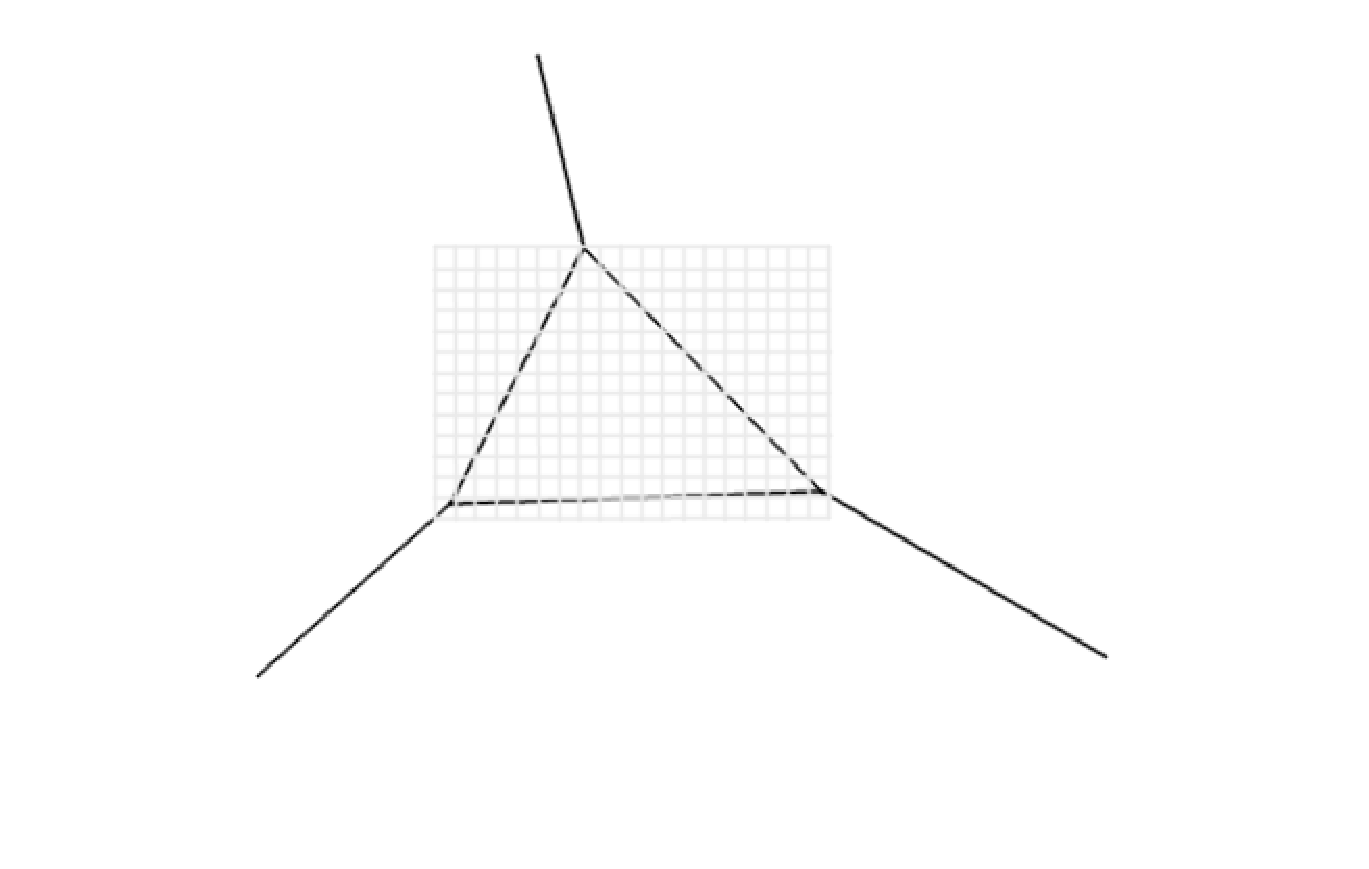
\includegraphics[scale=0.25]{../img/voxelize_1.eps}
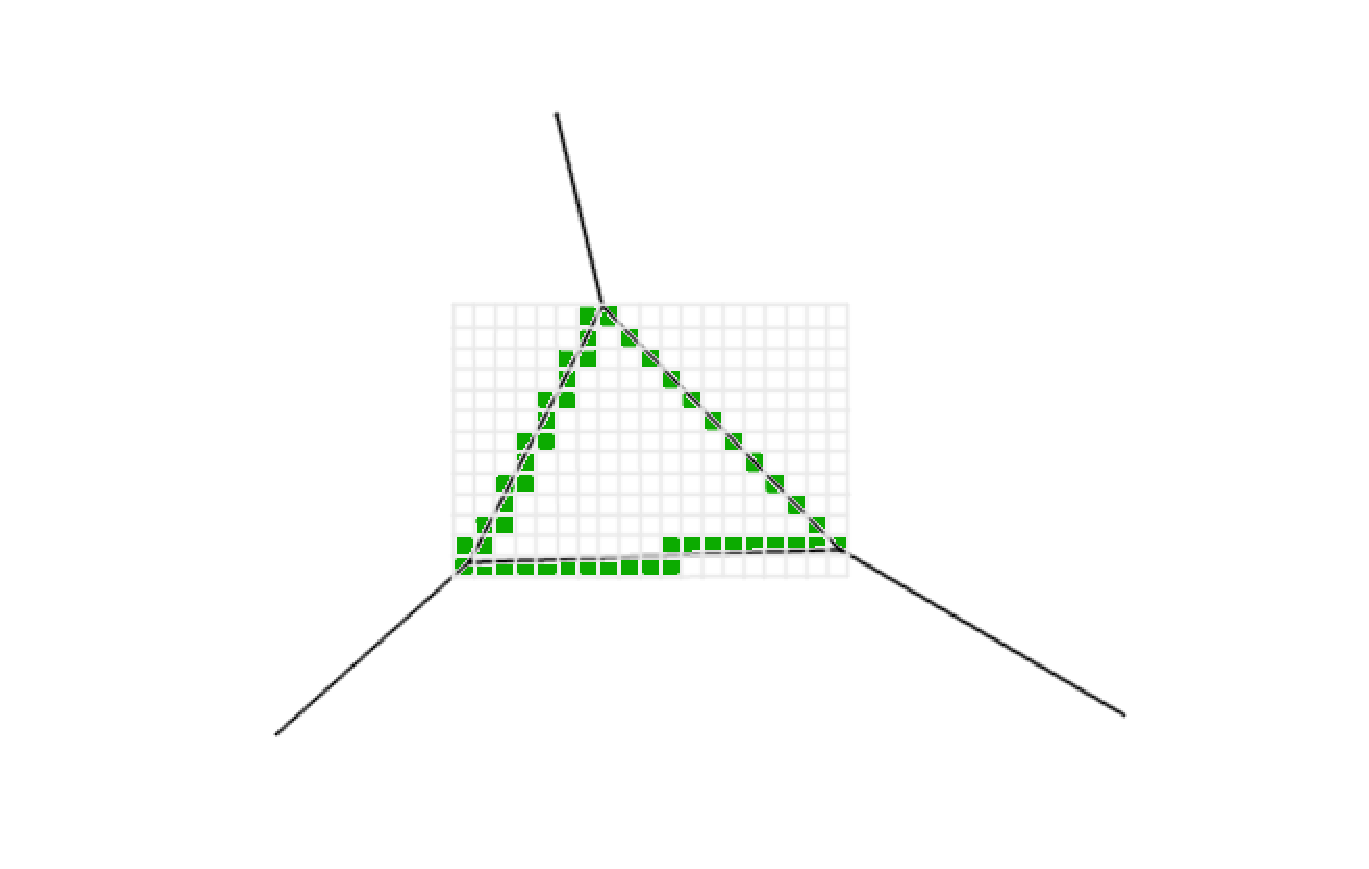
\includegraphics[scale=0.25]{../img/voxelize_2.eps}\\
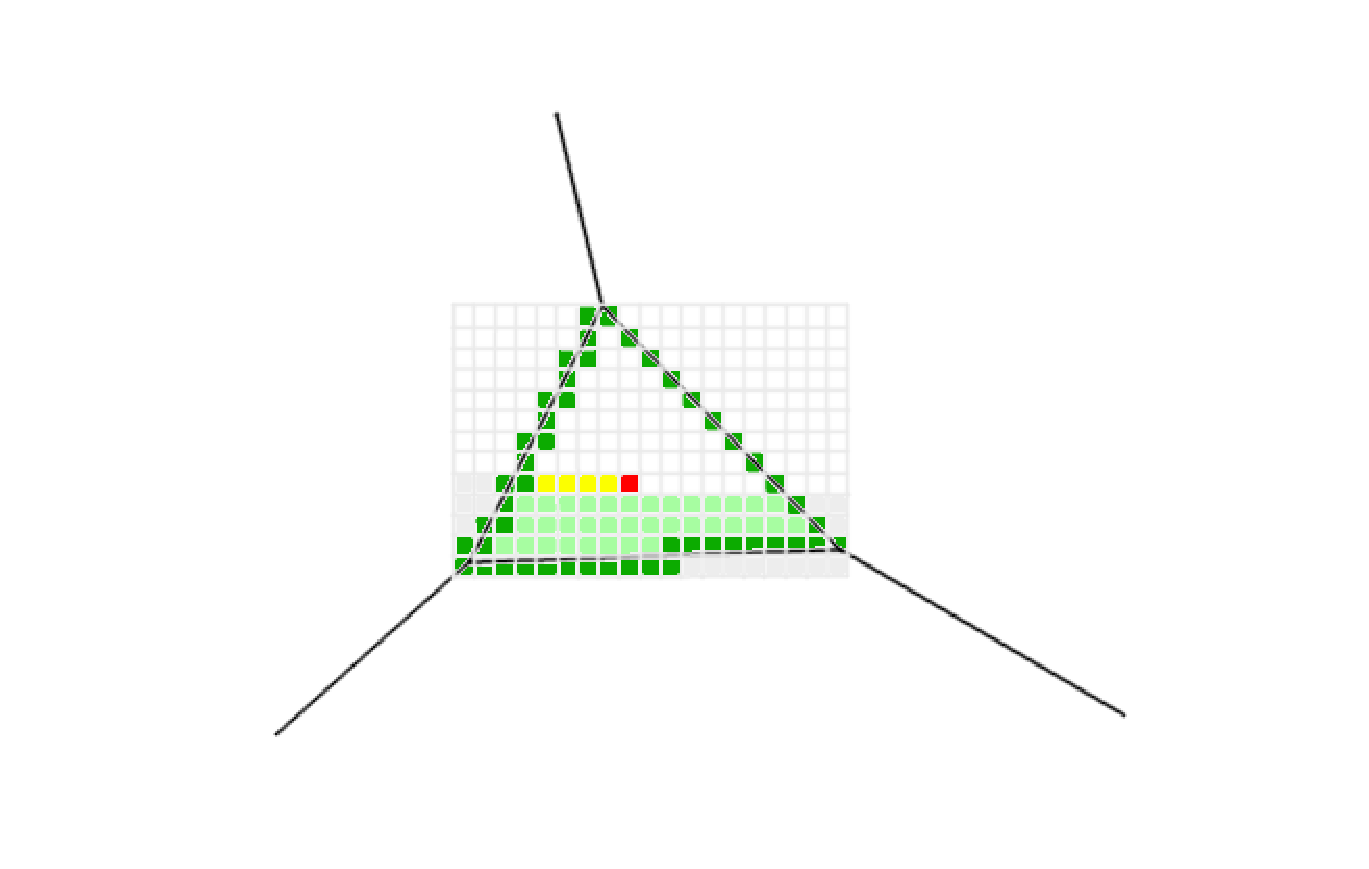
\includegraphics[scale=0.25]{../img/voxelize_3.eps}
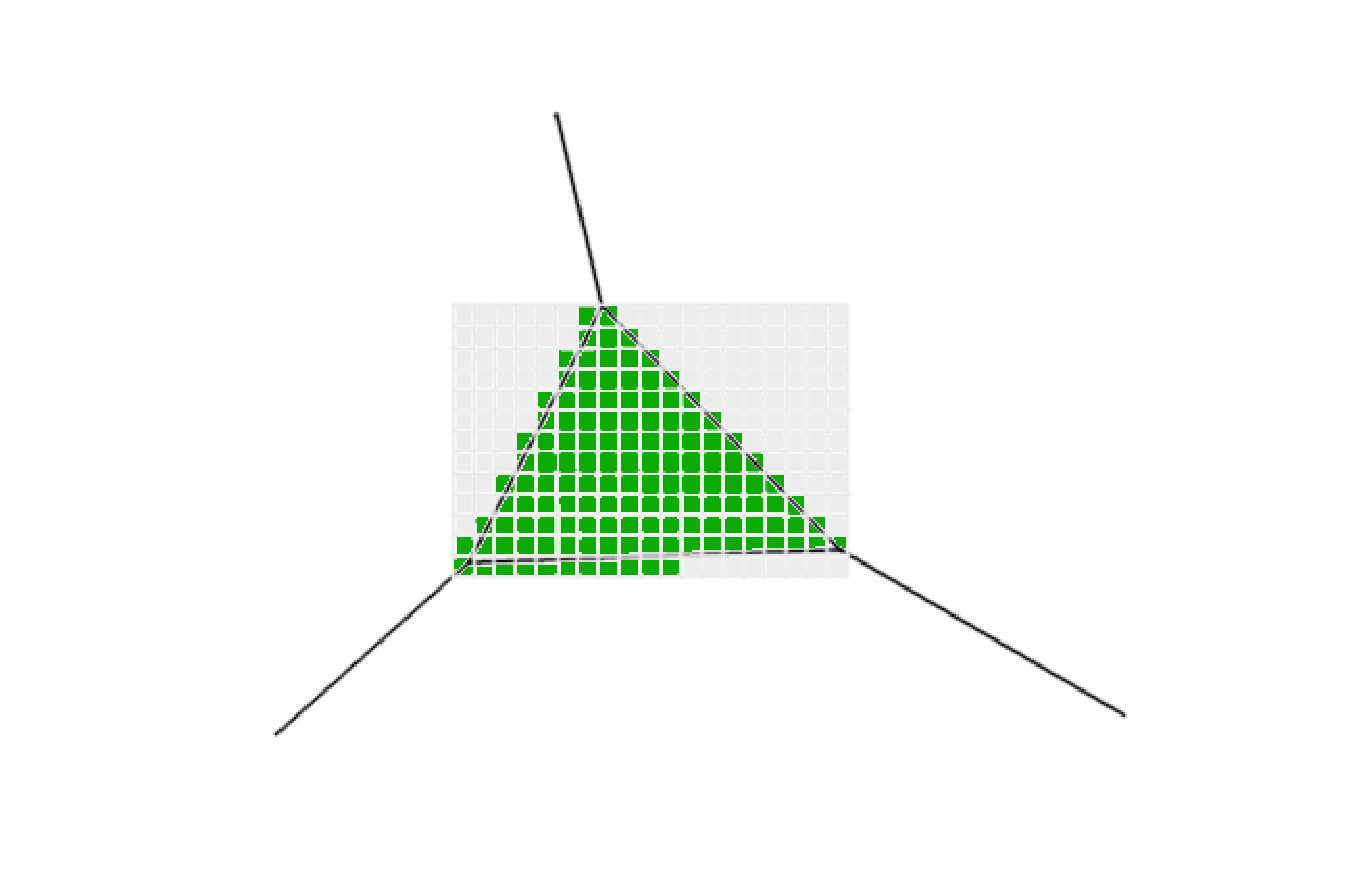
\includegraphics[scale=0.25]{../img/voxelize_4.eps}

\caption{Voxelization step-by-step}
\label{fig:voxelize}

\end{figure}

\begin{itemize}
\item On the pre-computed minimum boundary rectangle, start on the bottom and repeat for each line
\item In the line, start from an arbitrary side and process the elements consequently
\item After first crossing a rasterized edge, start filling the elements (entry the face)
\item After second crossing a rasterized edge, stop filling (leave the face).

\end{itemize}

In the second phase, the algorithm fills the elements inside the object. The only problem is to
determine whether the given voxel is inside or outside the object. As described above, the assumption of
starting with a line outside the enclosed area gives us the right method. The
bounding box will be needed in this case as well. If the object cannot be wrapped
the inside/outside property of element can not be determined.
